\begin{definitionbox}{Definition --- Metric Isometry}
\begin{definition}[Metric Isometry]\label{def:metric-isometry}
Let \((X,d_X)\) and \((Y,d_Y)\) be metric spaces.  A function
\(\phi:X\to Y\) is a \emph{metric isometry} if it preserves all pairwise
distances:
\[
  d_Y(\phi(a),\phi(b))=d_X(a,b)
\]
for all \(a,b\in X\).
\end{definition}
\end{definitionbox}

\begin{remark*}[Standard quantified statement]
\[
\phi\text{ is a metric isometry}
\quad\Longleftrightarrow\quad
\forall a,b\in X{:}\ d_Y(\phi(a),\phi(b))=d_X(a,b).
\]
\end{remark*}

\begin{remark*}[Predicate reading]
\[
\phi\text{ preserves metric distance from }X\text{ to }Y
\]
means that every pairwise distance in \(X\) is unchanged after applying
\(\phi\).
\end{remark*}

\begin{remark*}[Interpretation]
A metric isometry embeds one metric space into another without changing any
distance.  It preserves the metric structure, not merely the underlying set.
\end{remark*}

\LeanFormalizes{def:metric-isometry}{lra-lean}{LRA.VolumeIV.MetricSpaces.MetricIsometry.Isometry}{IsMetricIsometry}{statement}

\begin{dependencies}
\begin{itemize}
  \item \hyperref[def:metric-space]{Definition: Metric Space}
\end{itemize}
\end{dependencies}

\begin{definitionbox}{Definition --- Injective Map}
\begin{definition}[Injective Map]\label{def:injective-map}
A function \(\phi:X\to Y\) is \emph{injective} if
\[
  \phi(a)=\phi(b)\Longrightarrow a=b
\]
for all \(a,b\in X\).
\end{definition}
\end{definitionbox}

\begin{remark*}[Standard quantified statement]
\[
\phi\text{ is injective}
\quad\Longleftrightarrow\quad
\forall a,b\in X{:}\ \phi(a)=\phi(b)\Longrightarrow a=b.
\]
\end{remark*}

\begin{remark*}[Predicate reading]
\[
\phi\text{ is injective}
\]
means that equality of outputs forces equality of inputs.
\end{remark*}

\begin{remark*}[Interpretation]
Injectivity says that the function does not identify distinct input points.
\end{remark*}

\LeanFormalizes{def:injective-map}{lra-lean}{LRA.VolumeIV.MetricSpaces.MetricIsometry.Isometry}{IsInjectiveMap}{statement}

\begin{dependencies}
\begin{itemize}
  \item \hyperref[def:metric-isometry]{Definition: Metric Isometry}
\end{itemize}
\end{dependencies}

\begin{theorembox}{Theorem}
\begin{theorem}[Metric Isometries Are Injective]\label{thm:metric-isometries-injective}
Every metric isometry is injective.
\hyperref[prf:metric-isometries-injective]{\textit{Go to proof.}}
\end{theorem}
\end{theorembox}

\begin{remark*}[Standard quantified statement]
\[
\phi\text{ is a metric isometry}
\Longrightarrow
\phi\text{ is injective}.
\]
\end{remark*}

\begin{remark*}[Interpretation]
If two points have the same image under an isometry, then their image distance
is zero.  Distance preservation makes their original distance zero, so the
metric identity axiom forces the two points to be equal.
\end{remark*}

\LeanFormalizes{thm:metric-isometries-injective}{lra-lean}{LRA.VolumeIV.MetricSpaces.MetricIsometry.Isometry}{isMetricIsometry_injective}{checked}

\begin{dependencies}
\begin{itemize}
  \item \hyperref[def:metric-isometry]{Definition: Metric Isometry}
  \item \hyperref[def:injective-map]{Definition: Injective Map}
  \item \hyperref[def:metric-on-set]{Definition: Metric}
\end{itemize}
\end{dependencies}

\begin{theorembox}{Theorem}
\begin{theorem}[Positive and Negative Open Rays Are Isometric]
\label{thm:positive-negative-open-rays-isometric}
The map \(x\mapsto -x\) is a metric isometry from the positive open ray
\((0,\infty)\) onto the negative open ray \((-\infty,0)\), both with the
usual metric inherited from \(\mathbb{R}\).
\hyperref[prf:positive-negative-open-rays-isometric]{\textit{Go to proof.}}
\end{theorem}
\end{theorembox}

\begin{remark*}[Standard quantified statement]
\[
x\in(0,\infty)
\mapsto
-x\in(-\infty,0)
\quad\text{preserves distances.}
\]
\end{remark*}

\begin{remark*}[Interpretation]
Reflecting the real line across the origin preserves ordinary distance, so it
identifies the positive and negative open rays as the same metric shape.
\end{remark*}

\begin{figure}[htbp]
\centering
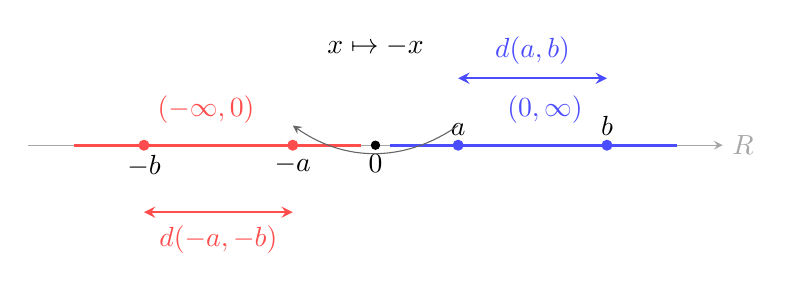
\begin{tikzpicture}[x=1.05cm,y=1cm,>=stealth]
  \draw[->,gray!70] (-4.2,0) -- (4.2,0) node[right] {\(\mathbb{R}\)};
  \fill[black] (0,0) circle (1.7pt);
  \node[below] at (0,0) {\(0\)};

  \draw[blue!70,very thick] (0.18,0) -- (3.65,0);
  \draw[red!70,very thick] (-3.65,0) -- (-0.18,0);
  \node[blue!70] at (2.05,0.45) {\((0,\infty)\)};
  \node[red!70] at (-2.05,0.45) {\((-\infty,0)\)};

  \foreach \x/\lab in {1/a,2.8/b}
  {
    \fill[blue!70] (\x,0) circle (2pt);
    \node[above] at (\x,0) {\(\lab\)};
    \fill[red!70] (-\x,0) circle (2pt);
    \node[below] at (-\x,0) {\(-\lab\)};
  }

  \draw[<->,blue!70,thick] (1,0.85) -- (2.8,0.85);
  \node[blue!70] at (1.9,1.2) {\(d(a,b)\)};
  \draw[<->,red!70,thick] (-2.8,-0.85) -- (-1,-0.85);
  \node[red!70] at (-1.9,-1.2) {\(d(-a,-b)\)};

  \draw[->,black!60] (1,0.25) to[bend left=35] (-1,0.25);
  \node at (0,1.25) {\(x\mapsto -x\)};
\end{tikzpicture}

\caption{The reflection \(x\mapsto -x\) preserves pairwise distances, so the
positive and negative open rays are isometric with the inherited real-line
metric.}
\label{fig:positive-negative-rays-isometry}
\end{figure}

\LeanFormalizes{thm:positive-negative-open-rays-isometric}{lra-lean}{LRA.VolumeIV.MetricSpaces.MetricIsometry.Isometry}{positiveOpenRay_isMetricIsometry_negativeOpenRay}{checked}

\begin{dependencies}
\begin{itemize}
  \item \hyperref[def:metric-isometry]{Definition: Metric Isometry}
  \item \hyperref[def:real-line-euclidean-distance]{Definition: Euclidean Distance on \(\mathbb{R}\)}
\end{itemize}
\end{dependencies}

\begin{definitionbox}{Definition --- Isometric Copy}
\begin{definition}[Isometric Copy]\label{def:isometric-copy}
Let \(X\) be a metric space and let \(Z\subseteq Y\), where \(Y\) is a metric
space.  The subset \(Z\) is an \emph{isometric copy} of \(X\) if there is a
metric isometry \(\phi:X\to Y\) whose range is \(Z\).
\end{definition}
\end{definitionbox}

\begin{remark*}[Standard quantified statement]
\[
Z\text{ is an isometric copy of }X
\Longleftrightarrow
\exists\phi:X\to Y{:}\ \phi\text{ is a metric isometry}
\land \phi(X)=Z.
\]
\end{remark*}

\begin{remark*}[Interpretation]
An isometric copy is a subset that can be reached from the original space by a
distance-preserving parametrization.
\end{remark*}

\LeanFormalizes{def:isometric-copy}{lra-lean}{LRA.VolumeIV.MetricSpaces.MetricIsometry.Isometry}{IsometricCopy}{statement}

\begin{dependencies}
\begin{itemize}
  \item \hyperref[def:metric-isometry]{Definition: Metric Isometry}
\end{itemize}
\end{dependencies}
